%----------------------------------------------------------------------------
\chapter{A multiprocesszoros OpenCL környezet}
%----------------------------------------------------------------------------

\section{OpenCL architektúrája}
	Az Open Computing Language (OpenCL) keretrendszer \cite{opencl}
	általános modellt, magas szintű programozási interfészt és hardware
	absztrakciót nyújt a fejlesztőknek adat- vagy feladat párhuzamos számítások gyorsítására különböző
	számítóegységen (CPU, GPU, FPGA, DSP, \ldots).
	A hárdvergyártók implementálják az OpenCL szabványt, ami által saját platformot
	hoznak létre. Egy ilyen platformon belüli eszközök alatt főként GPU-kat, de
	CPU-kat és FPGA-t \ldots is értünk.
	OpenCL keretrendszerben történő programozás során két programot kell írnunk.
	Az egyik a kernel, ami az eszközön futatott szálra fog leképeződni.
	A másik a gazda processzoron (host-on) futó host-program, ami elvégzi az I/O műveleteket,
	a probléma összeállítását, a memória allokálást, az argumentumok beállítását
	illetve a kernel meghívását az eszközön.
	A kernel futása végeztével a host-program kiolvassa az eszközből
	a kívánt eredményt.
	
	\begin{figure}[!h]
		\centering
		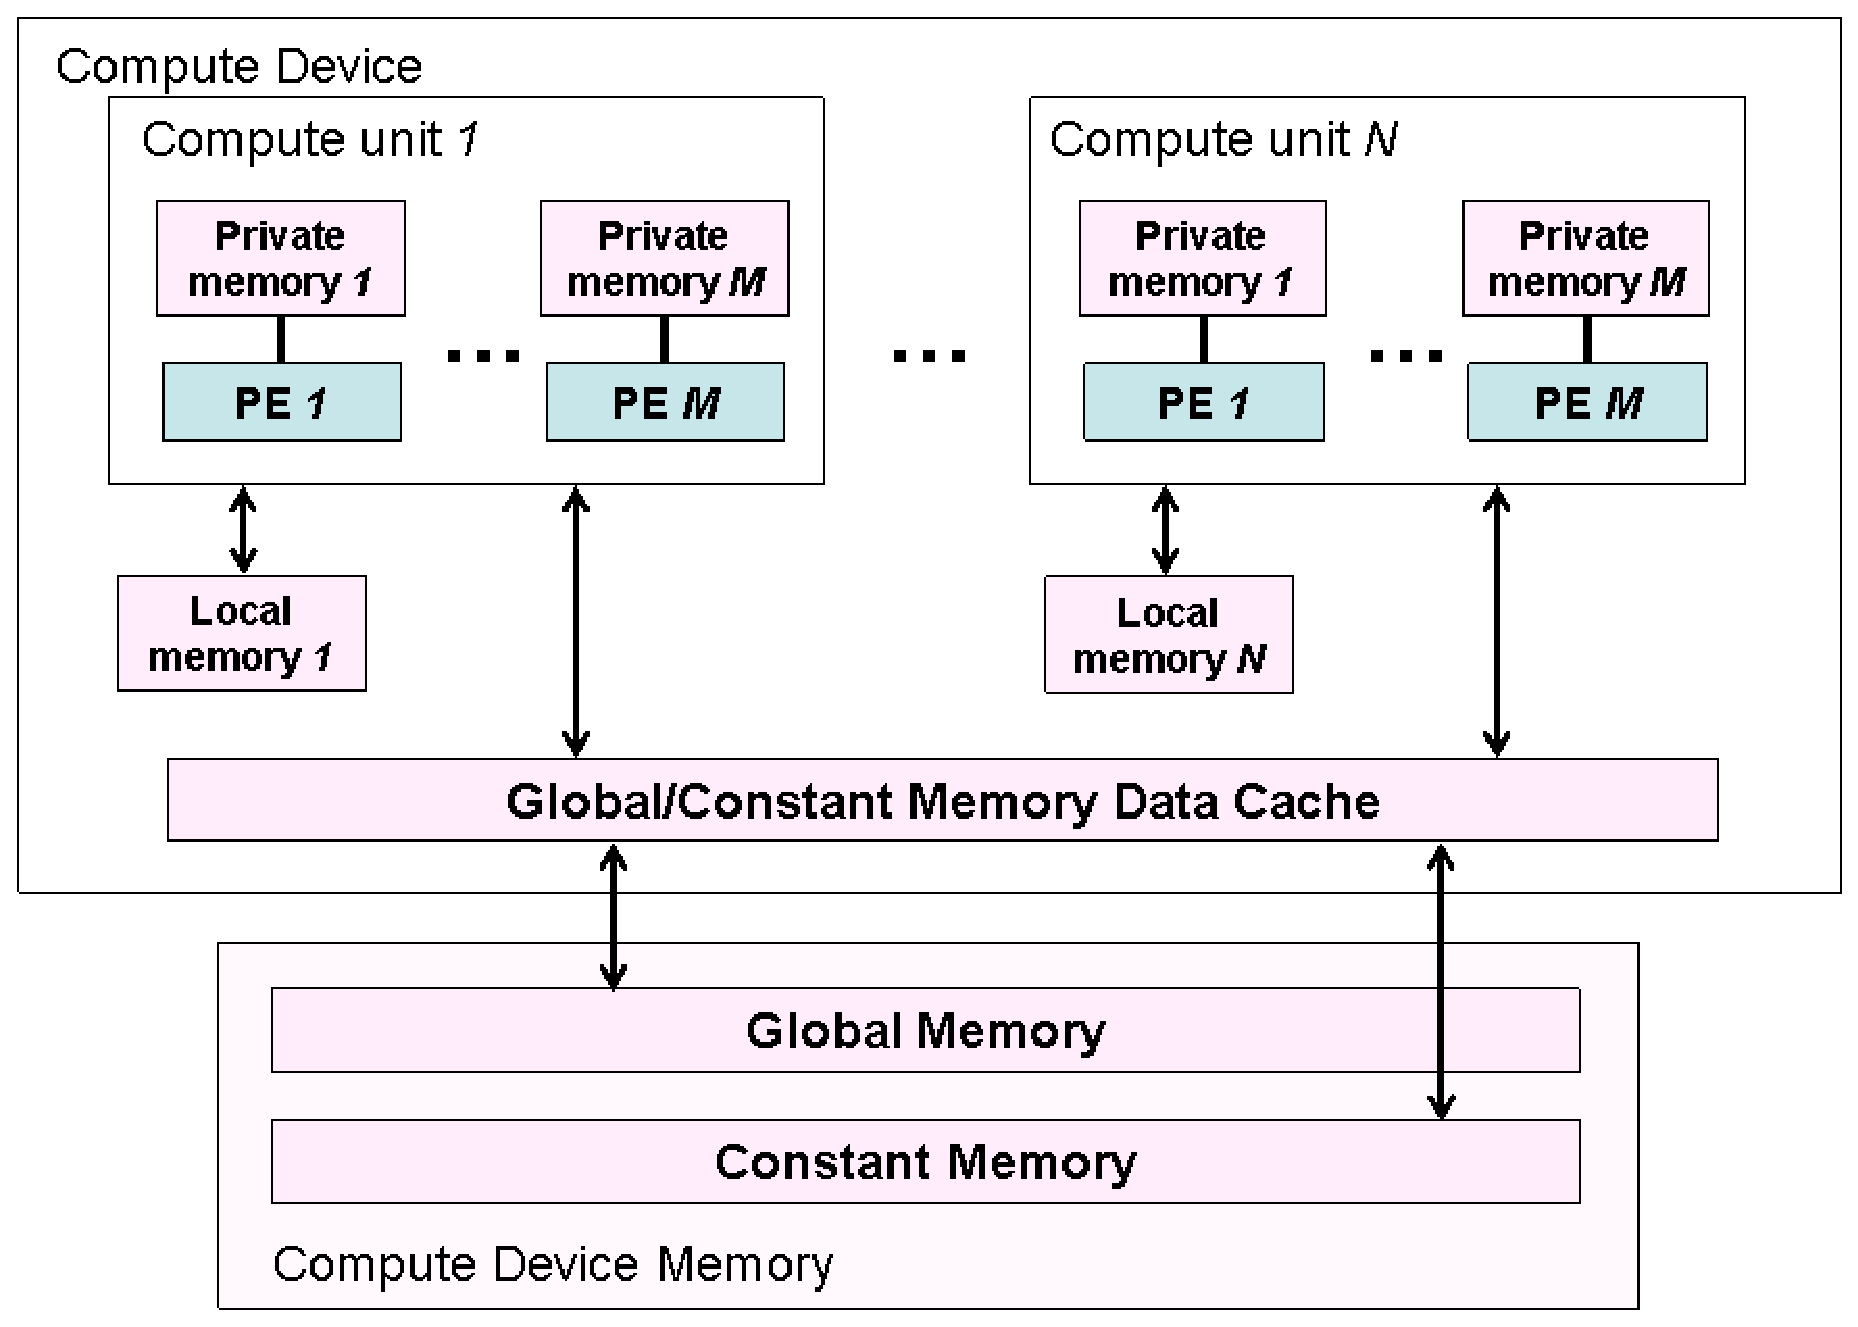
\includegraphics[width=0.6\columnwidth]{figures/eps/device.eps}
		\caption{OpenCL device architektúra (forrás: \cite{opencl})} 
		\label{fig:device} 
	\end{figure}
	Az eszközök multiprocesszoros architektúrával és ezek kiszolgálására képes
	memória architektúrával rendelkeznek, amit a \ref{fig:device} ábra vázol.
	Egy eszköz több compute unit-ot (processzor-magot) tartalmaz.
	Az OpenCL négy memória szintet különböztet meg, amikre a
	következőképpen hivatkozik:
	\begin{itemize}
		\item \emph{Regiszterek:} Private memory,
		\item \emph{Chipen belüli memória (cache):} Local memory,
		\item \emph{Chipen kívüli memória:} Global memory és Constant Memory.
	\end{itemize}
	A regiszterek és lokális memória kis méretűnek és gyors elérésűnek modható, míg
	a globális memória nagynak de lassú elérésűnek.
	A memóriákra megkötésként szolgál, hogy ki allokálhat, írhat és olvashat
	belőle. A \ref{table:mem} táblázatban látható ezen jogosultságok.
	\begin{table}[!h]
	%\renewcommand{\arraystretch}{1.3}
	% if using array.sty, it might be a good idea to tweak the value of
	% \extrarowheight as needed to properly center the text within the cells
	\caption{OpenCL memória szintek}
	\label{table:mem}
	\centering
	% Some packages, such as MDW tools, offer better commands for making tables
	% than the plain LaTeX2e tabular which is used here.
	\begin{tabular}{l|l|l|l|l}
			 & Global memory & Constant mem. & Local mem. & Private mem.\\ \hline
		Host & Dinamikusan R/W & Din. R/W & Din. R/W & \\
		Kernel & R/W & Statikusan R & Satik. R/W & Statik. R/W\\
		Sebesség & Lassú & Gyors & Gyors & Regiszter\\
		Méret & $1$ Gbyte $<$ & $\sim64$ Kbyte& $\sim16$ Kbyte & $<1$ Kbyte
	\end{tabular}
	\end{table}
	
	Ahhoz, hogy a rendszerben rejlő teljesítményt kihozzuk három fontos kérdést
	kell a szimulátor magjának implementálásakor megválaszolnunk:
	\begin{itemize}
		\item \emph{Mennyit?}: Tisztában kell lennünk az aktuális
		memória fogyasztással és a szükséges memóriamérettel.
		\item \emph{Honnan-hova?}: Fontos, hogy a lehető legközelebb legyen az adat
		a processzor-maghoz.
		\item \emph{Mikor?}: Mivel a memória művelet alatt a futtatott kernel nem
		dolgozik, így átadja a helyét egy másiknak. (Ez Direct Memory Access (DMA)
		blokk létezése allatt igaz). Ennek a megfelelő szinkronizációjával nagyobb
		kihasználtság érhető el (load balance).
	\end{itemize}
	
	
\section{OpenCL programozási modell}
	
	A programozási modell középpontjában a kontextus áll, ami az OpenCL
	osztálydiagrammján \ref{fig:class} figyelhető meg.
	A futtatáshoz szükséges, hogy a kontextushoz platformot, majd azon belül
	eszközt, az eszközhöz programot (kernelt) és memóriát rendeljünk.
	\begin{figure}[!h]
		\centering
		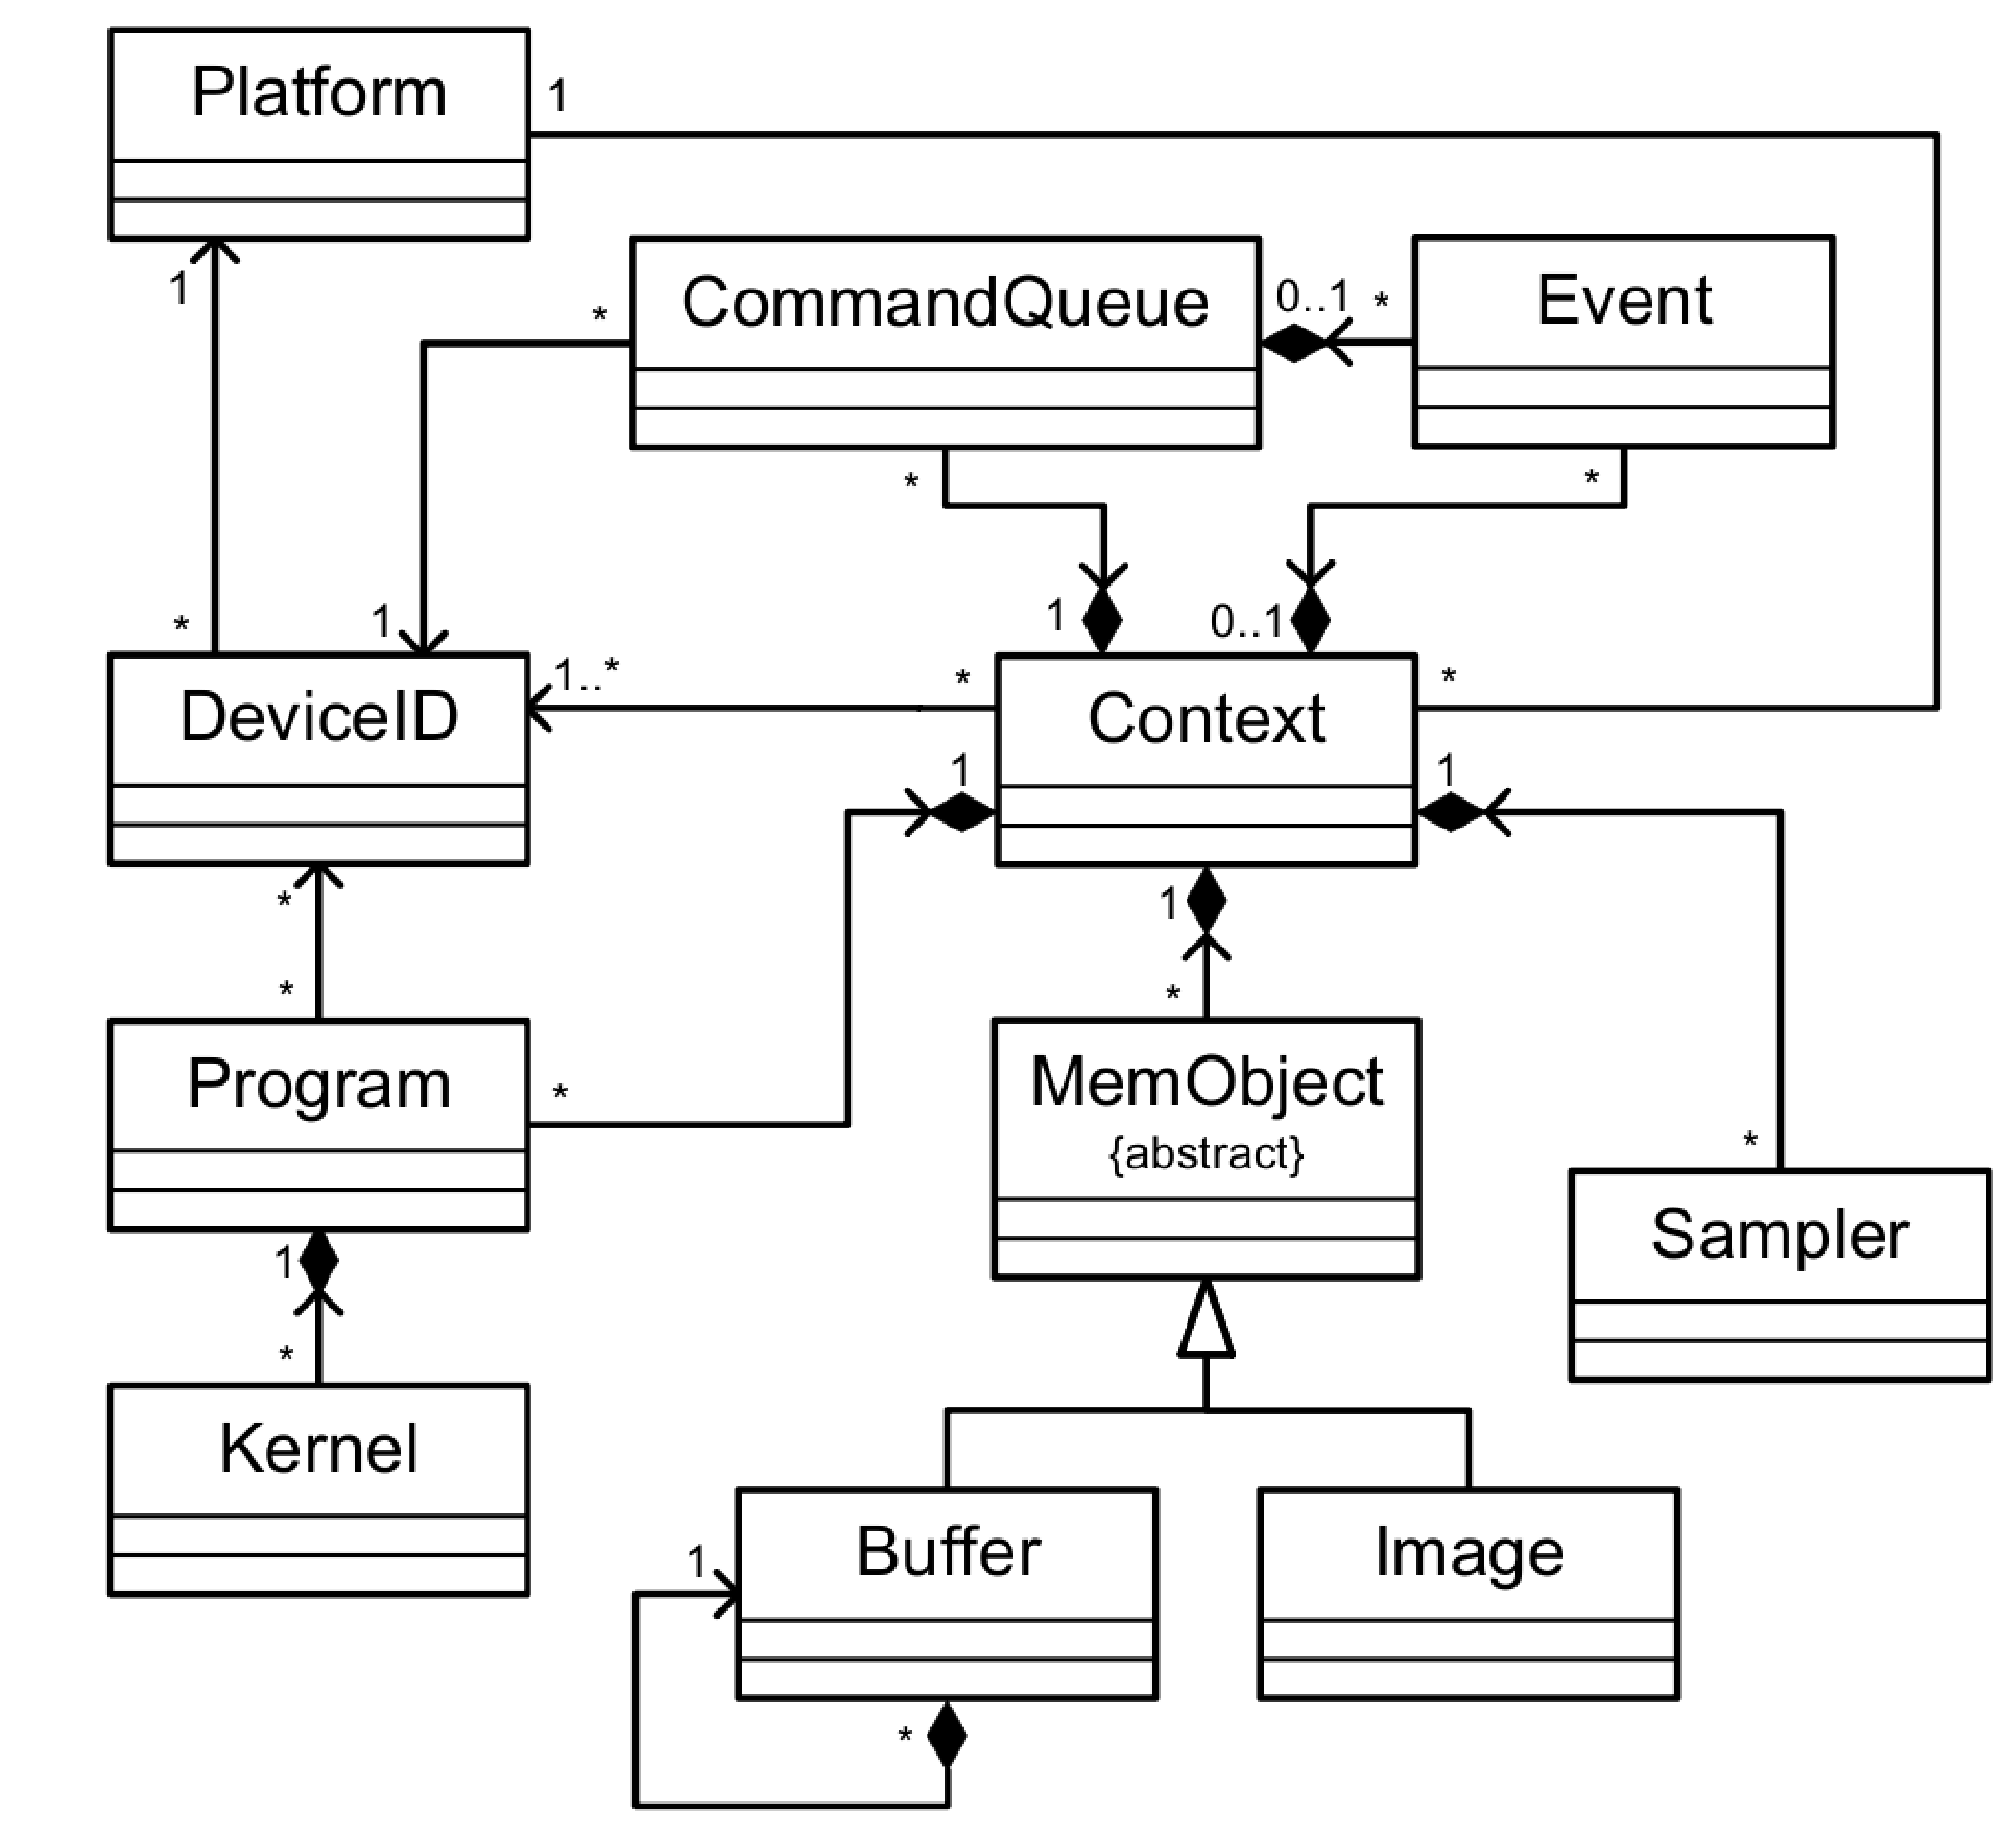
\includegraphics[width=0.6\columnwidth]{figures/eps/context.eps}
		\caption{OpenCL context osztálydiagrammja (forrás: \cite{opencl})} 
		\label{fig:class} 
	\end{figure}
	Figyelembe kell vennünk azt a megkötést, hogy csak az egy platformon belüli
	eszközök programozhatóak heterogén módon. Például: Intel platform esetén
	lehetséges CPU-t, processzorkártyát és Intel-es GPU-t programozni.
	
	A programozással megoldandó problémát kétféleképpen lehetséges a feldolgozó
	egységekhez (work-item) avagy processzorokhoz rendelni:
	adat parallel módon vagy taszk parallel módon.
	Adat parallel módon (\ref{fig:data_parallel} ábra) a feldolgozandó adat egy
	egységéhez rendelünk egy feldolgozó egységet. Fontos figyelembe venni az eszköz korlátos
	számú feldolgozó egységének számát. Ha nem elég a feldolgozó egysége akkor a
	feladat megfelelő partícionálásával lehetséges kordában tartani a szükséges
	erőforrás számát.
	Taszk parallel módot (\ref{fig:task_parallel} ábra) olyan esetben célszerű
	használna, ha a bemenet dinamikus mérete a futási időben rendkívül változik
	illetve a végrehajtandó feladat lezán függenek össze.
	
	\begin{figure*}[!h]
		\centering
		\subfloat[Adat parallel]{
			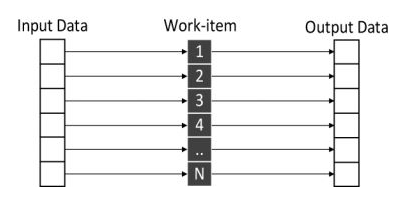
\includegraphics[width=0.45\columnwidth]{figures/eps/data.eps}%
			\label{fig:data_parallel}
		}
		\hfil
		\subfloat[Taszk parallel]{
			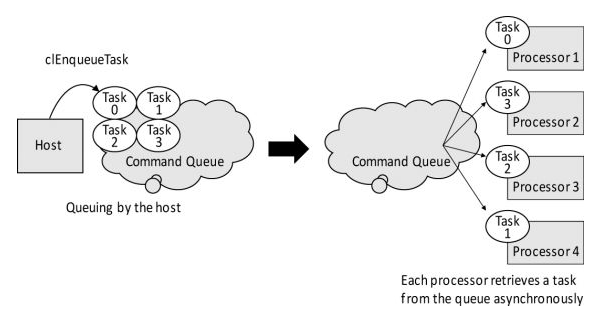
\includegraphics[width=0.45\columnwidth]{figures/eps/task.eps}%
			\label{fig:task_parallel}
		}
		\caption{Feladat hozzárendelése work-item-hez (processzorhoz)}
		\label{fig:parallel}
	\end{figure*}
	A processzor-magok megfelelő kihasználtságának elérése végett több ezer
	work-item virtuális osztozik rajta.
	Továbbá ezen work-item-eket work-group-okba rendezzük.
	
	A work-itemeket jelen pillanatban az OpenCL specifikációja szerint 3 dimenziós work-group-ba tudjuk
	rendezni. Egy példát láthatunk egy work-item indexének a globális és lokális megfelelőjére a
	követekző \ref{fig:ndrange} ábrán.
	
	\begin{figure}[!h]
		\centering
		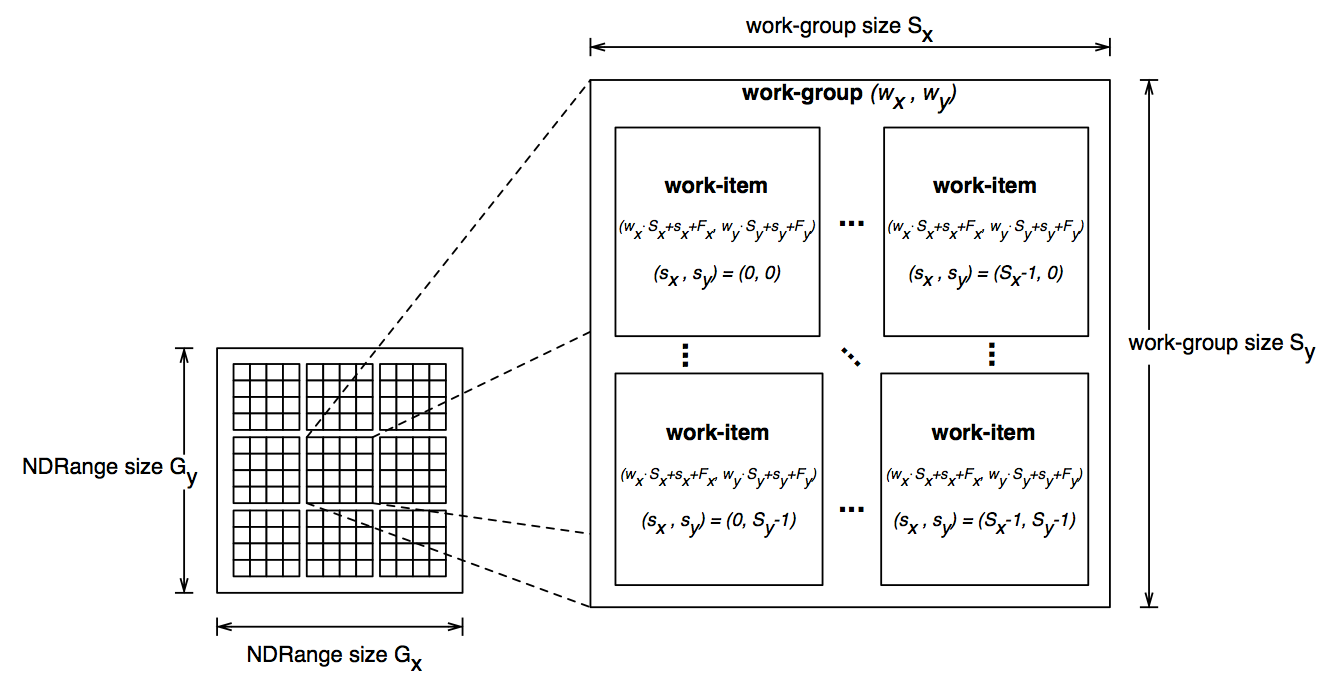
\includegraphics[width=0.9\columnwidth]{figures/eps/ndrange.eps}
		\caption{2D-s work-item-ek work-group-ba rendezése és indexelése (forrás: \cite{opencl})} 
		\label{fig:ndrange} 
	\end{figure}

	A work-group-okba rendezés a lokális memória jogusultsága miatt érdekes.
	Konkrétan egy work-group-ba tartozó összes work-item azonos lokális memórián
	osztozik.
	Ennek a következménye az, hogy adat parallel módú feldolgozás esetén
	az egymásra ható adatokhoz tartozó work-item-eket egy work groupba kell
	rendelnünk.
	Ha ez nem lehetséges, akkor a globális memóriához kell fordulnunk.
	A globális memória avagy a bank szervezésű külső (off-chip) memóriák
	hozzáférési ideje relatíve nagy így ezek használatát lehetőleg el kell kerülni
	és a programozónak kell ``cahchelni" a lokális memóriába.
	
	Mivel a work-item-ek konkurrensen hajtódnak végre, így az általuk közösen elérhető memóriákra
	(globális, lokális) nézve versenyhelyzetben vannak.
	Az OpenCL ezt a problémát a laza memóriamodell használatával oldja meg. Az alkalmazott
	szinkronizáció egy korlátot tesz a programban, amit csak akkor léphet át, ha az összes többi
	work-item az azonos work-group-ban ezta a korlátot már elérte. Erre a \texttt{barrier(FLAG)}
	függvényhívás szolgál. Fontos megjegyezni, hogy ez a szinkronizáció csak egy adott
	work-group-on belül történik, a work-group-ok közötti szinkronizációra nincs lehetőség. 
	
	\begin{center}
	Összefoglalva nagy hangsúlyt kell a memóriaszervezésre fordítani, hogy a
	processzormag megfelelően legyenek az adatokkal táplálva.
	\end{center}


\section{Futási környezet bemutatása}
	A következő eszközök teljesítményét vizsgálom:
	\begin{itemize}
		\item A laptopomban található \textbf{Intel Core i5 M520} processzor,
		\item A laptopomban található kis teljesítményű \textbf{nVidia GT330M} videókártya,
		\item Asztali PC-ben található \textbf{Intel Xeon CPU},
		\item Asztali PC-ben található \textbf{Intel Xeon Phi} co-processzor \cite{phi,mic }. 
	\end{itemize}
	Ezen eszközök legjelentősebb paraméterei a \ref{table:envs} táblázat tartalmazza.
	
	\begin{table}[!h]
	%\renewcommand{\arraystretch}{1.3}
	% if using array.sty, it might be a good idea to tweak the value of
	% \extrarowheight  as needed to properly center the text within the cells
	\setlength{\extrarowheight}{8pt}
	\caption{Használandó eszközök összehasonlítása}
	\label{table:envs}
	\centering
	\footnotesize
	% Some packages, such as MDW tools, offer better commands for making tables
	% than the plain LaTeX2e tabular which is used here.
	\begin{tabular}{ l | r | r | r | r}
		 & Intel Core i5 & nVidia GT330M & Intel Xeon & Xeon PHI \\ \hline
		MAX COMPUTE UNITS & $4$ & $6$ & $8$ & $224$\\
		MAX CLOCK FREQUENCY & 2400 & 1265 & 3000 & 1100\\
		MAX WORK GROUP\_SIZE & $8192$ & $512$ & $8192$ & $8192$ \\ \hline\hline
		GLOBAL MEM SIZE & $\sim 4Gbyte$ & $1Gbyte$ & $8Gbyte$ & $\sim 4.5Gbyte$\\
		%MAX\_CONSTANT\_BUFFER\_SIZE & $131072$ & $65536$ & $131072$ & $131072$\\
		LOCAL MEM SIZE & $32 Kbyte$ & $16 Kbyte$ & $32 Kbyte$ & $32 Kbyte$\\
	\end{tabular}
	\end{table}
	
	Az összehasonlíthatóság végett a legkissebb memóriájú eszközre fogom a problémát skálázni, ami a
	GT330M videókártya. A többi eszköz memóriája jóval nagyobb, így a kód könnyen portolható rájuk.

\section{Implementációhoz szükséges megfontolások}

	Ezen feladatrészek méretét egy paraméter állításával lehet változtati és az
	implementált algoritmus ettől generikusan függ.
	Emellett az interpoláció mértéke is generikusan paraméterrel állítható.
	Az algoritmus generikusságát csupán a futási időben történő dinamikus memória
	allokációval lehetséges megvalósítani. A korábban említettek végett (\ref{table:mem} táblázat)
	az allokáció csak a ``host'' programban történhet.

\section{Memória szervezés}
\subsection{Csak globális memória használata}
	Az algoritmus pszeudó kódjának direkt leképezése esetén a ``host''-on
	allokálunk memóriát a ``device'' globális memóriájában.
	Majd a megfelelő adatokat ide másoljuk és a kernel is itt ír és olvas.
	A problémát a globális memória nagy hozzáférési ideje jelenti, ami miatt sok
	``work-item'' tétlenül a memóriára fog várakozni.
	Ilyenkor az egy mérési pontra vonatkoztatott szimulációs idő a
	referenciánál is lassabb.
\subsection{Globális memória és adott esetben lokális memória használata}
	Kis erőfeszítéssel nagy javulást lehet elérni, ha a mérési ponthoz tartozó
	szimulációs tér éppen belefér a lokális memóriába.
	Tehát, mielött az \ref{eq:2} szerinti iteratív megoldót futtatnánk először a
	globális memóriából a lokális memóriába töltjük át a kérdéses pontokat, majd
	számolunk rajt és a végén visszatöltjük a globális memóriába.
	E javítással a referenciával azonos sebességet tudunk elérni.
\subsection{Globális memória és minden adódó alkalomkor a lokális memória használata}
	Nagyobb erőfeszítést igényel, hogy a globális memórival való kommunikációt a
	lokális memória közbeékelésével tegyünk minden alkalomkor.
	Ezt úgy lehet felfogni, mintha a globális memóriát lokális memória méretű
	kvantumokban tudnám csak elérni.
	Ekkor nagy odafigyelést kíván a memóriacímzés megfelelő prgramozása, de
	eredményképp gyorsulás elérhető.
	
	\noindent
	\begin{center}
	Összegezve elmondható, hogy az aktuálisan használt adat tárolását a lehető
	legközelebb kell tartani a processzor-maghoz.
	\end{center}






